\subsubsubsection{Merging Histories}

\todo{merging histories}

\def\blkGrp#1{\save [].[r]!C="g#1"*[F.]\frm{}\restore}%
\def\blkGrpM[#1]#2{\save [].[#1]!C="g#2"*[F.]\frm{}\restore}%

\subparagraph{simple}

\begin{equation*}
    \xyMChains{
        & & & \xBB{1a} \arm[ld] & & \xBB{2a} \arm[ll] \\
        & \cdots & \xBBi \arm[l] & & & & \xBB3 \arm[lu] \ars[lld] \\
        & & & & \xBB{1b} \arm[llu] & \\
        & \xyTimeHoriz{rrrrrr} &&&&&&
    }
\end{equation*}

\begin{equation*}
    \xyMChains{
        % & & & \xBB{1a} \arm[ld] & & \xBB{2a} \arm[ll] \\
        & \cdots \arm[r]
            & \xBBi \arm[r]
            & \xBB{1a} \arm[r]
            & \xBB{2a} \arm[r]
            & \xyBDraft{\BB{1b}} \arm[r] \blkGrp1
            & \xBB3 \\
        & \xyLabelHoriz{Execution Order}{0pt}{rrrrrr}{r30pt} &&&&&&
        % \save "1,6"."1,7"*[F.]\frm{}
        % \restore
    }
\end{equation*}

\subparagraph{bit complex}

\begin{equation*}
    \xyMChains{
        & & & \xBB{1a} \arm[ld] & \xBB{2a} \arm[l] \ars[ldd] \\
        & \cdots & \xBBi \arm[l] & & & & \xBB3 \arm[llu] \ars[ld] \\
        & & & \xBB{1b} \arm[lu] & & \xBB{2b} \ars[ll] \arm[lluu] \\
        & \xyTimeHoriz{rrrrrr} &&&&&&
    }
\end{equation*}

\begin{equation*}
    \xyMChains{
        & \cdots \arm[r]
            & \xBBi \arm[r]
            & \xBB{1a} \arm[r]
            & \xyBDraft{\BB{1b}} \arm[r] \blkGrp1
            & \xBB{2a} \arm[r]
            & \xyBDraft{\BB{2b}} \arm[r] \blkGrp2
            & \xBB3 \\
        & \xyLabelHoriz{Execution Order}{0pt}{rrrrrr}{r30pt} &&&&&&
    }
\end{equation*}

\subparagraph{multiparent}

\begin{equation*}
    \xyMChains{
        & & & & \xBB{2a} \arm[ld] \\
        & \cdots & \xBBi \arm[l] & \xBB{1} \arm[l] & \xBB{2b} \arm[l] & \xBB3 \arm[lu]_1 \ars[l]_2 \ars[ld]^3 \\
        & & & & \xBB{2c} \arm[lu] \\
        & \xyTimeHoriz{rrrrrr} &&&&&&
    }
\end{equation*}

\begin{equation*}
    \xyMChains{
        & \cdots \arm[r]
            & \xBBi \arm[r]
            & \xBB{1} \arm[r]
            & \xBB{2a} \arm[r]
            & \xyBDraft{\BB{2b}} \arm[r] \blkGrpM[rr]1
            & \xyBDraft{\BB{2c}} \arm[r]
            & \xBB3 \\
        & \xyLabelHoriz{Execution Order}{0pt}{rrrrrr}{r30pt} &&&&&&
    }
\end{equation*}

\subparagraph{block structure}

\begin{figure}
    \centering
    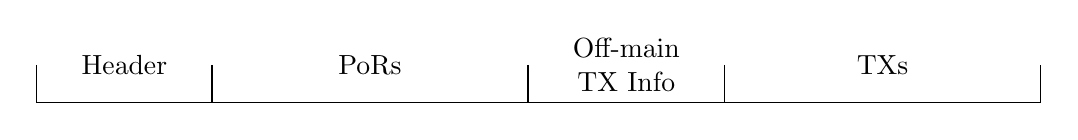
\begin{tikzpicture}[node distance=0cm]
        % \tikzstyle{n} = [draw, rectangle, solid, black, align=center, inner sep=10pt, minimum width=4cm, anchor=north]
        % \tikzstyle{tall} = [minimum height=2cm]

        % \node (header) [n] {header (\sim100 B)};
        % \node (refls) [n] at (header.south) {PoRs};
        % \node (uncles) [n] at (refls.south) {Off-main headers \\ and merkle roots};
        % \node (txs) [n] at (uncles.south) {Main TXs};
        % % \node (txs-body) [n, tall] at (refls.south) {
        % %     \node (prev-txs) [n, tall] {Sec Parents' Txs};
        % %     \node (txs) [n, tall] at (prev-txs.south) {Main Txs};
        % % };

        \tikzstyle{n} = [align=center, inner xsep=16pt, inner ysep=4pt, anchor=west]
        \tikzstyle{wide} = [minimum width=4cm]

        \node (hdr) [n] {Header};
        \node (pors) [n, wide] at (hdr.east) {PoRs};
        \node (offmain) [n] at (pors.east) {Off-main \\ TX Info};
        \node (txs) [n, wide] at (offmain.east) {TXs};

        \node (ml) at (hdr.west) {};
        \node (bl) at (offmain.south -| ml) {};
        \node (mr) at (txs.east) {};
        \node (br) at (bl -| mr) {};

        \draw (ml.center) -- (bl.center) -- (br.center) -- (mr.center);
        \draw (pors.west) -- (pors.west |- bl);
        \draw (offmain.west) -- (offmain.west |- bl);
        \draw (txs.west) -- (txs.west |- bl);

    \end{tikzpicture}
    \caption[short]{long cap}
\end{figure}

\subparagraph{Which State Roots are Accurate?}

When using a block-DAG that commits to state (e.g., a UTXO set), we've just seen that transactions in off-main blocks are only processed when they're \emph{still} valid.
For a transaction to be executed, it must be included in either a main chain block, \emph{or} an off-main block whilst not conflicting with prior transactions.

Additional  status can change between the time it's included in an off-main block and when it's executed by a main-chain block, the state root of that block

only main-chain state roots and txs are reliable.
off-main state roots are totally wrong,
and off-main transactions might be executed but we can't be sure.
only main-chain blocks and state roots matter
